%=========================================================
\section{P2 --- ¿Puede YOLOv8 localizar y separar morfológicamente las ráfagas FHSS?}
\label{sec:bloque_yolo}

\subsection{Planteamiento del experimento}
\label{sec:p2_planteamiento}

El segundo experimento reformula el reconocimiento de señales como un problema de detección de objetos. En lugar de asignar una etiqueta global a cada espectrograma, el modelo debe generar cajas delimitadoras sobre las ráfagas individuales del plano tiempo-frecuencia y clasificar cada una como \emph{drone} (ráfaga OcuSync) o \emph{interference} (ráfaga WiFi/Bluetooth). Las etiquetas se generan con el auto-etiquetado descrito en la \cref{sec:autoetiquetado} (umbral percentil 99,8, etiquetado débil por captura), y el detector se configura según la \cref{sec:entrenamiento_yolo} (YOLOv8n, entrada 640×640, lote~16, sin aumentaciones geométricas).

Se realizan dos entrenamientos sobre el mismo dataset: una primera tanda de \num{15}~épocas como referencia inicial, y una segunda tanda de \num{60}~épocas como modelo final.

Las métricas de precisión, recall y mAP se definen en la \cref{subsec:diseno_evaluacion}. Conviene precisar aquí la distinción entre métricas globales y por clase: el \textbf{mAP@50 global} promedia la precisión media de cada clase activa sobre el conjunto de prueba; el \textbf{mAP@50 por clase} permite comparar directamente el rendimiento del detector sobre \emph{drone} frente a \emph{interference}. La \textbf{puntuación de confianza} (\emph{confidence score}) es el valor entre 0 y 1 que el modelo asigna a cada detección; se emplea como umbral de filtrado para controlar el equilibrio entre precisión y recall, y su elección óptima se determina a partir de la curva F1-confianza mostrada en los resultados.

\subsection{Resultados}
\label{sec:p2_resultados}

\paragraph{Evolución del entrenamiento.}

La \cref{fig:yolo_run02_results} muestra las curvas de pérdida y métricas de validación a lo largo de las \num{60}~épocas del modelo final.

\begin{figure}[htbp]
    \centering
    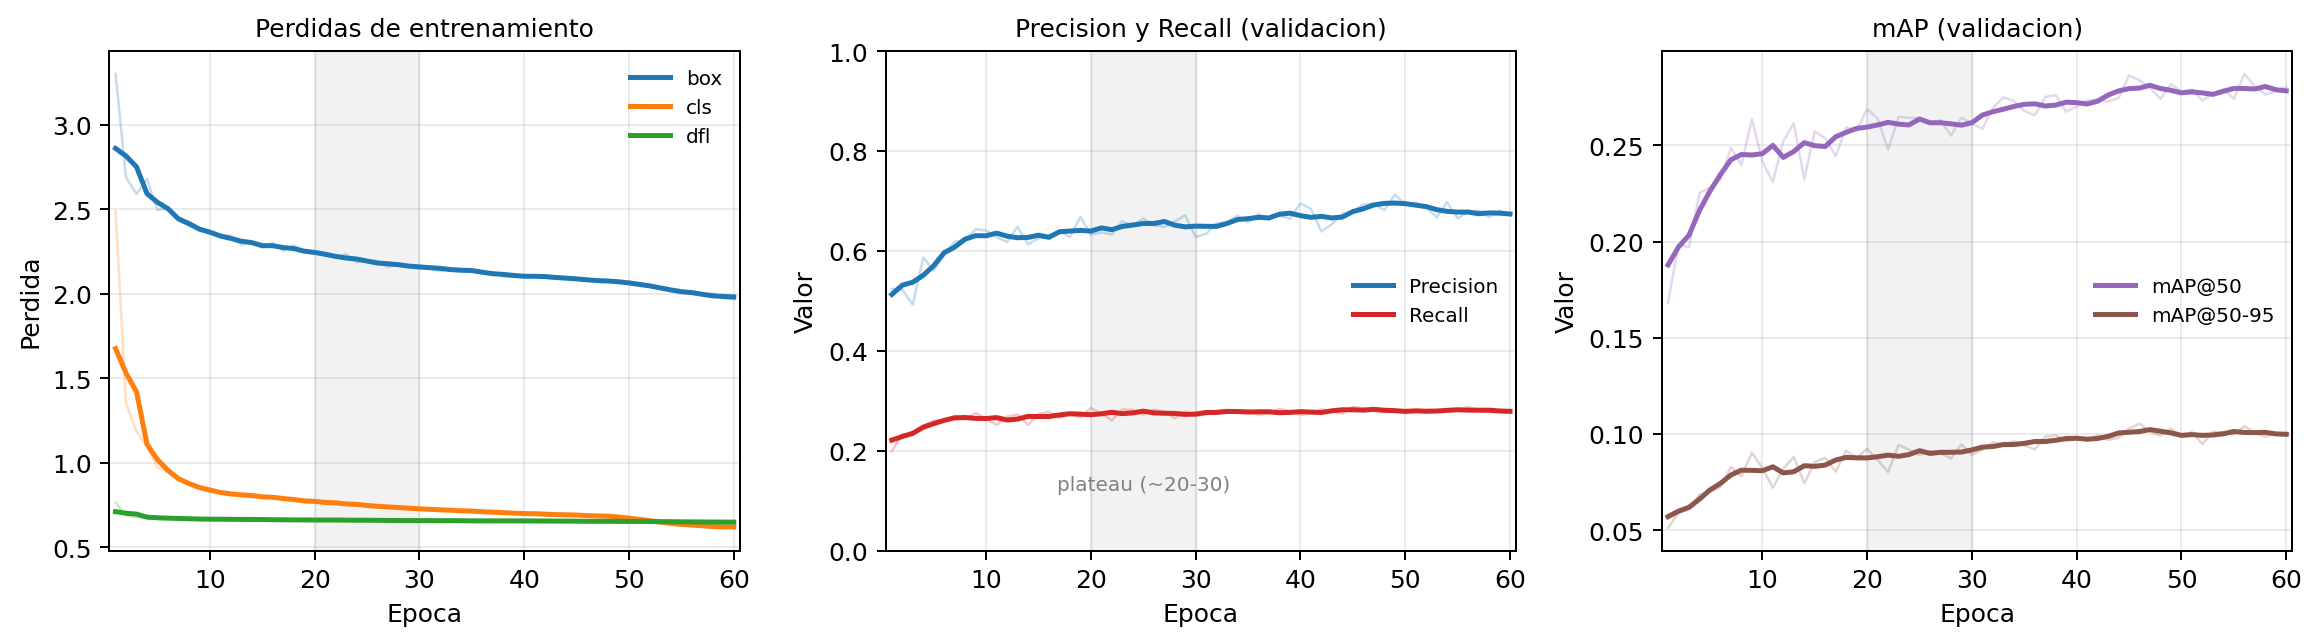
\includegraphics[width=\textwidth]{figuras/resultados/yolo_run02_curvas.png}
    \caption{Evolución del entrenamiento del detector YOLOv8n a lo largo de las \num{60}~épocas (tanda~2), resumida en tres paneles. Izquierda: las tres pérdidas de entrenamiento (box, cls, dfl) descienden de forma continua. Centro: la precisión y el recall de validación se estabilizan en una meseta aproximadamente entre las épocas 20 y 30 (banda sombreada). Derecha: el mAP@50 y el mAP@50-95 de validación siguen el mismo patrón; las épocas adicionales aportan una leve mejora de la precisión geométrica de las cajas (mAP@50-95) sin aumentar de forma significativa la cobertura (recall, mAP@50). En cada panel la línea tenue son los valores por época y la gruesa la tendencia suavizada.}
    \label{fig:yolo_run02_results}
\end{figure}

Las curvas muestran un comportamiento saludable: las pérdidas de entrenamiento descienden de forma continua y no hay señales de sobreajuste severo. Las métricas de validación se estabilizan entre las épocas~20 y~30 sin tendencia creciente clara a partir de ese punto. Esto indica que el límite del experimento no reside en la duración del entrenamiento, sino en la dificultad intrínseca del problema --- tamaño de las ráfagas en el espectrograma y ruido en el etiquetado automático ---, que las épocas adicionales no pueden superar.

\paragraph{Comparativa entre tandas.}

La \cref{tab:comparativa_epochs} compara los resultados de test de ambas tandas de entrenamiento.

\begin{table}[htbp]
\centering
\caption{Comparativa de resultados sobre el conjunto de prueba entre la tanda de \num{15}~épocas y la de \num{60}~épocas.}
\label{tab:comparativa_epochs}
\begin{tabular}{lccc}
\toprule
\textbf{Métrica} & \textbf{15 épocas} & \textbf{60 épocas} & \textbf{Diferencia} \\
\midrule
Precisión global        & 0,748 & 0,760 & +0,012 \\
Recall global           & 0,395 & 0,391 & $-$0,004 \\
mAP@50 global           & 0,386 & 0,388 & +0,002 \\
mAP@50-95 global        & 0,195 & 0,203 & +0,008 \\
mAP@50 drone            & 0,571 & 0,575 & +0,004 \\
mAP@50-95 drone         & 0,333 & 0,348 & +0,015 \\
mAP@50 interference     & 0,201 & 0,201 & $\pm$0,000 \\
mAP@50-95 interference  & 0,056 & 0,058 & +0,002 \\
\bottomrule
\end{tabular}
\end{table}

La tanda de \num{60}~épocas aporta una mejora marginal en la mayoría de métricas, siendo más apreciable en mAP@50-95 para \emph{drone} (+0,015). Esto es coherente con las curvas de la \cref{fig:yolo_run02_results}: las épocas adicionales refinan la localización geométrica de las cajas de dron sin aumentar el número de ráfagas detectadas.

\FloatBarrier
\paragraph{Separabilidad entre clases: matriz de confusión.}

La matriz de confusión normalizada constituye el resultado más relevante del experimento para responder a P2. En la matriz, las filas corresponden a las clases reales y las columnas a las clases predichas (incluyendo \emph{background}). Los valores de la diagonal indican la tasa de acierto de cada clase; los valores fuera de la diagonal entre dos clases activas indican confusión cruzada entre ellas; los valores en la columna \emph{background} indican ráfagas reales no detectadas.

\begin{figure}[htbp]
    \centering
    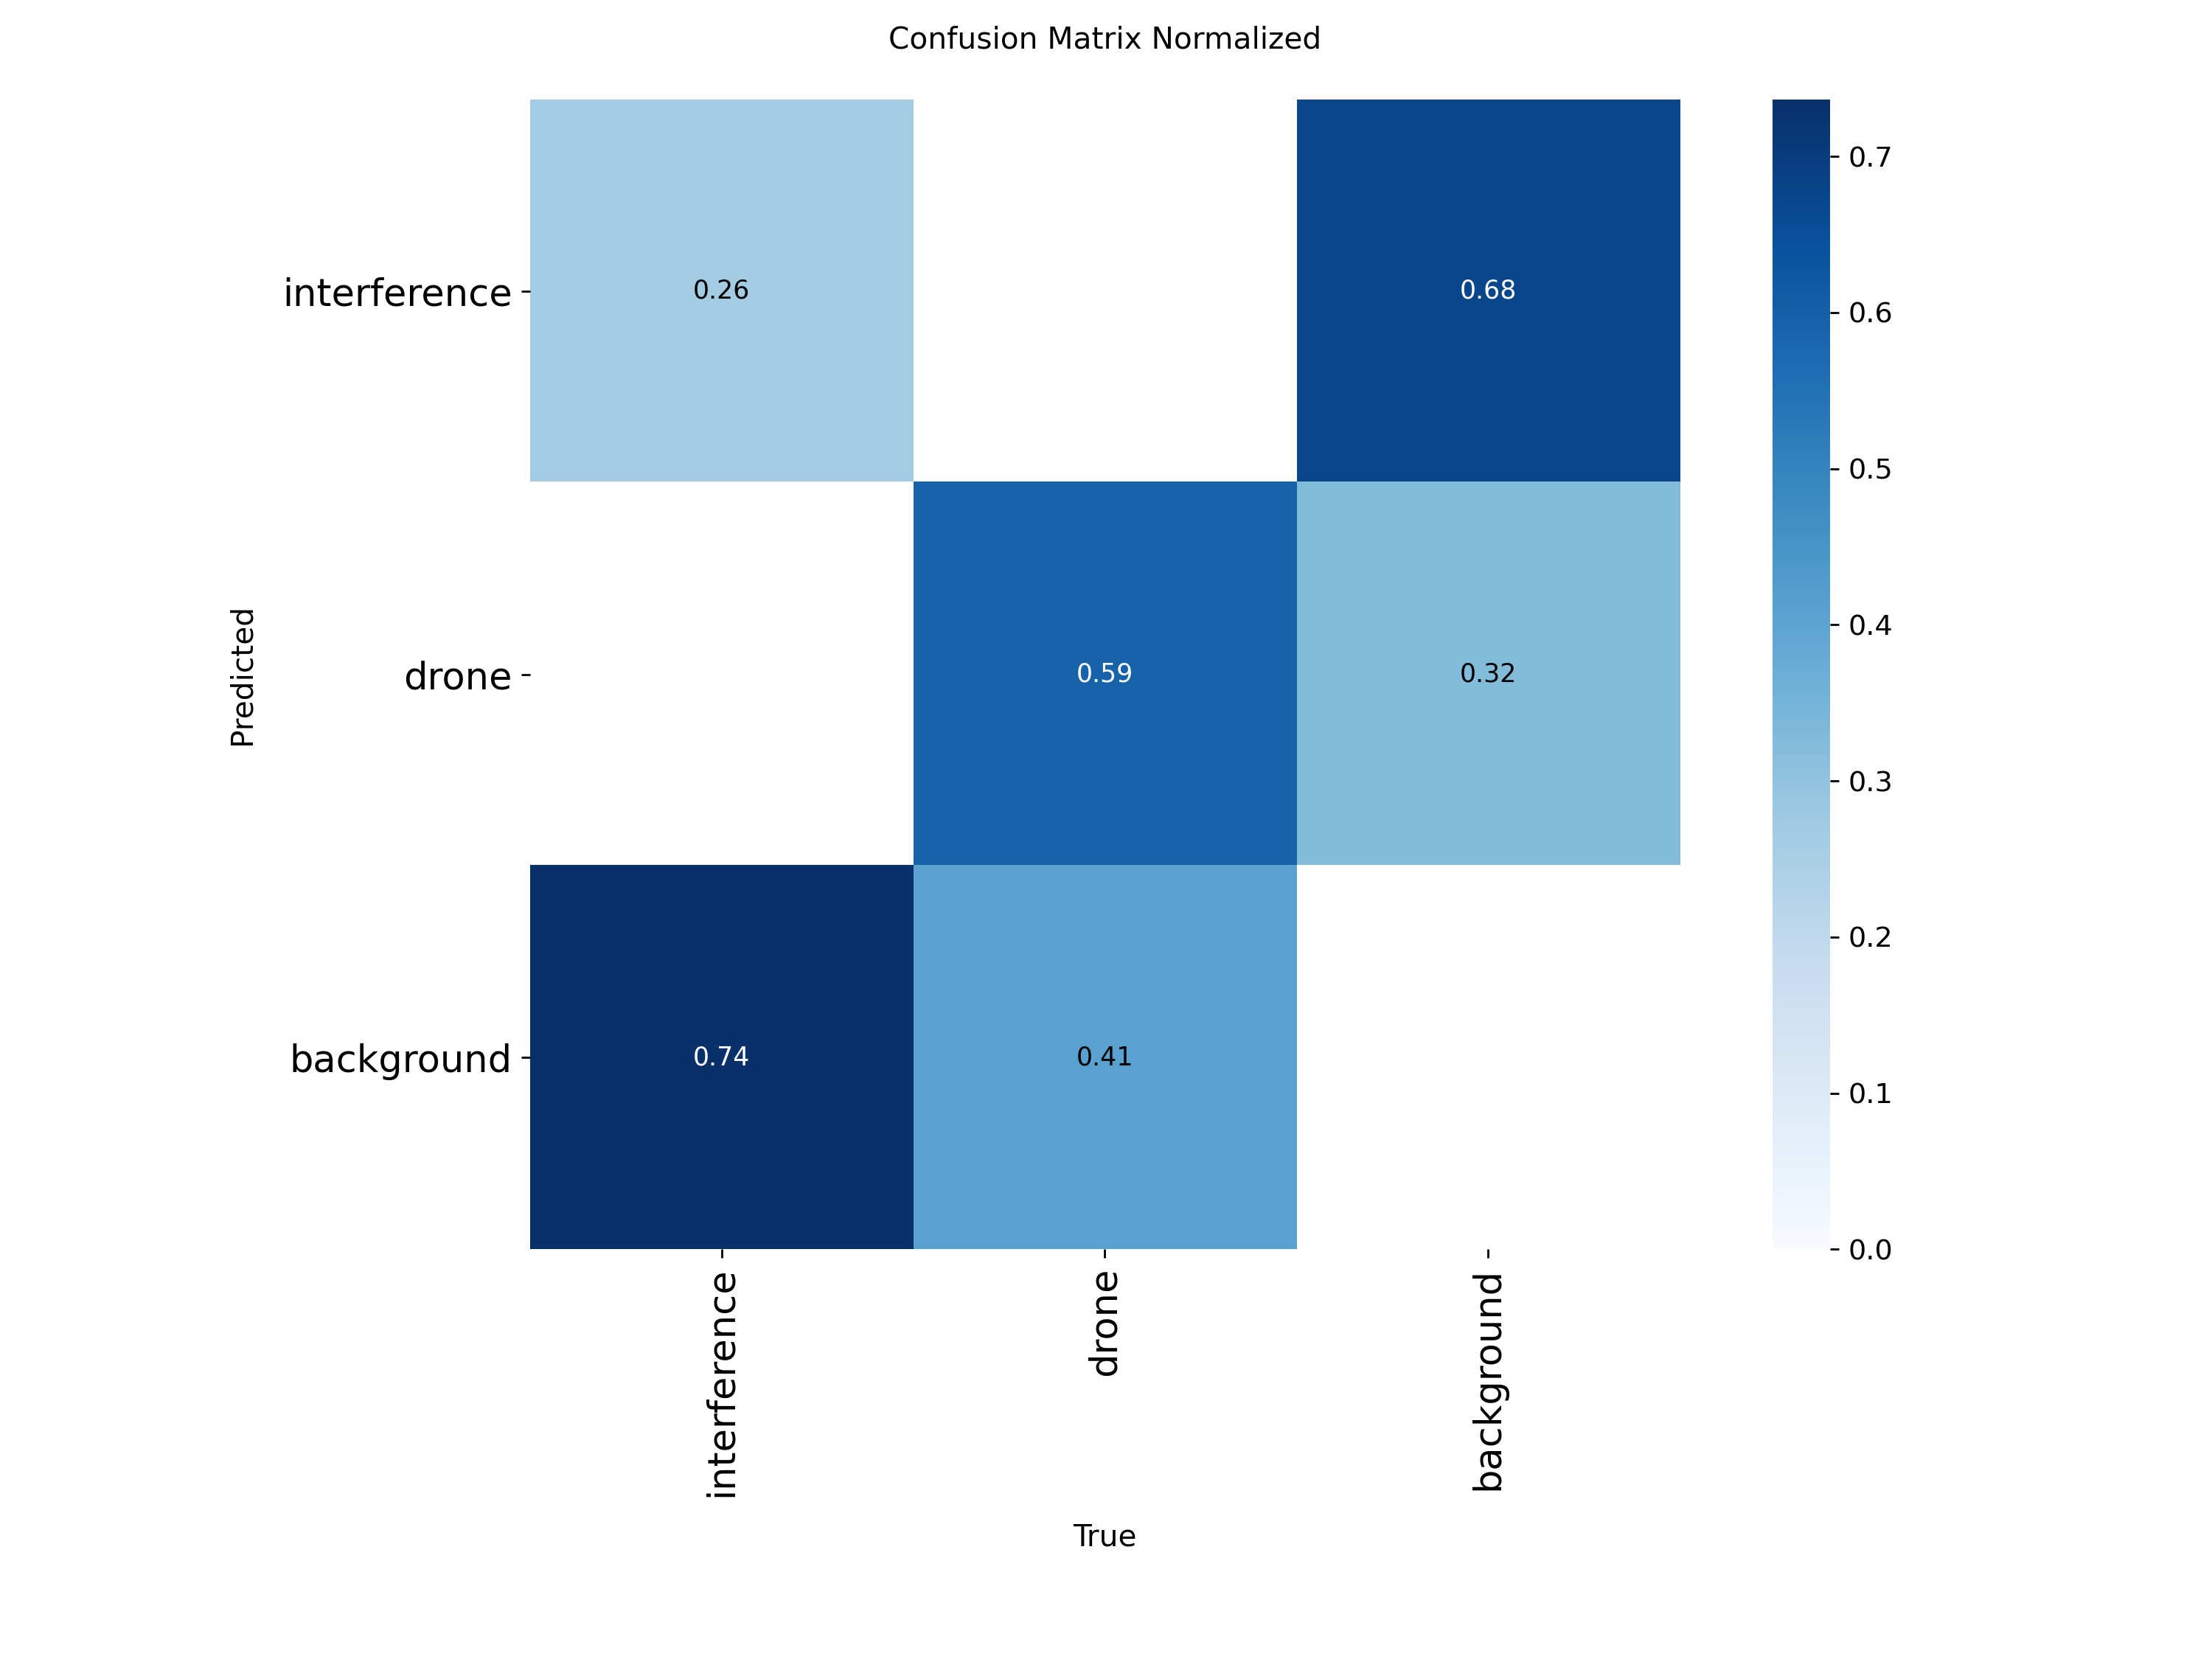
\includegraphics[width=0.75\textwidth]{figuras/resultados/confusion_matrix_normalized.png}
    \caption{Matriz de confusión normalizada del detector YOLOv8n sobre el conjunto de prueba. No se observa confusión cruzada entre \emph{drone} e \emph{interference}: cuando el modelo emite una predicción positiva, la clase asignada es correcta. Los errores son íntegramente falsos negativos (ráfagas reales asignadas a \emph{background}).}
    \label{fig:confusion_matrix_normalized}
\end{figure}

La \cref{fig:confusion_matrix_normalized} revela el resultado central del experimento: no existe confusión cruzada entre \emph{drone} e \emph{interference}. Ninguna ráfaga real de OcuSync es clasificada como interferencia, y ninguna ráfaga de interferencia es clasificada como señal de dron. Las tasas de confusión cruzada son ambas 0,00. Los errores son íntegramente falsos negativos: la tasa de detección a nivel de caja es de 0,42 para \emph{drone} y de 0,18 para \emph{interference}, con el complemento asignado a \emph{background}.

\FloatBarrier
\paragraph{Curvas precisión-recall y F1-confianza.}

La \cref{fig:box_pr_curve} muestra la curva precisión-recall del detector para ambas clases. La curva resume el equilibrio entre precisión y recall al variar el umbral de confianza: a umbrales altos el modelo es más selectivo (mayor precisión, menor recall); a umbrales bajos acepta más detecciones (mayor recall, menor precisión).

\begin{figure}[htbp]
    \centering
    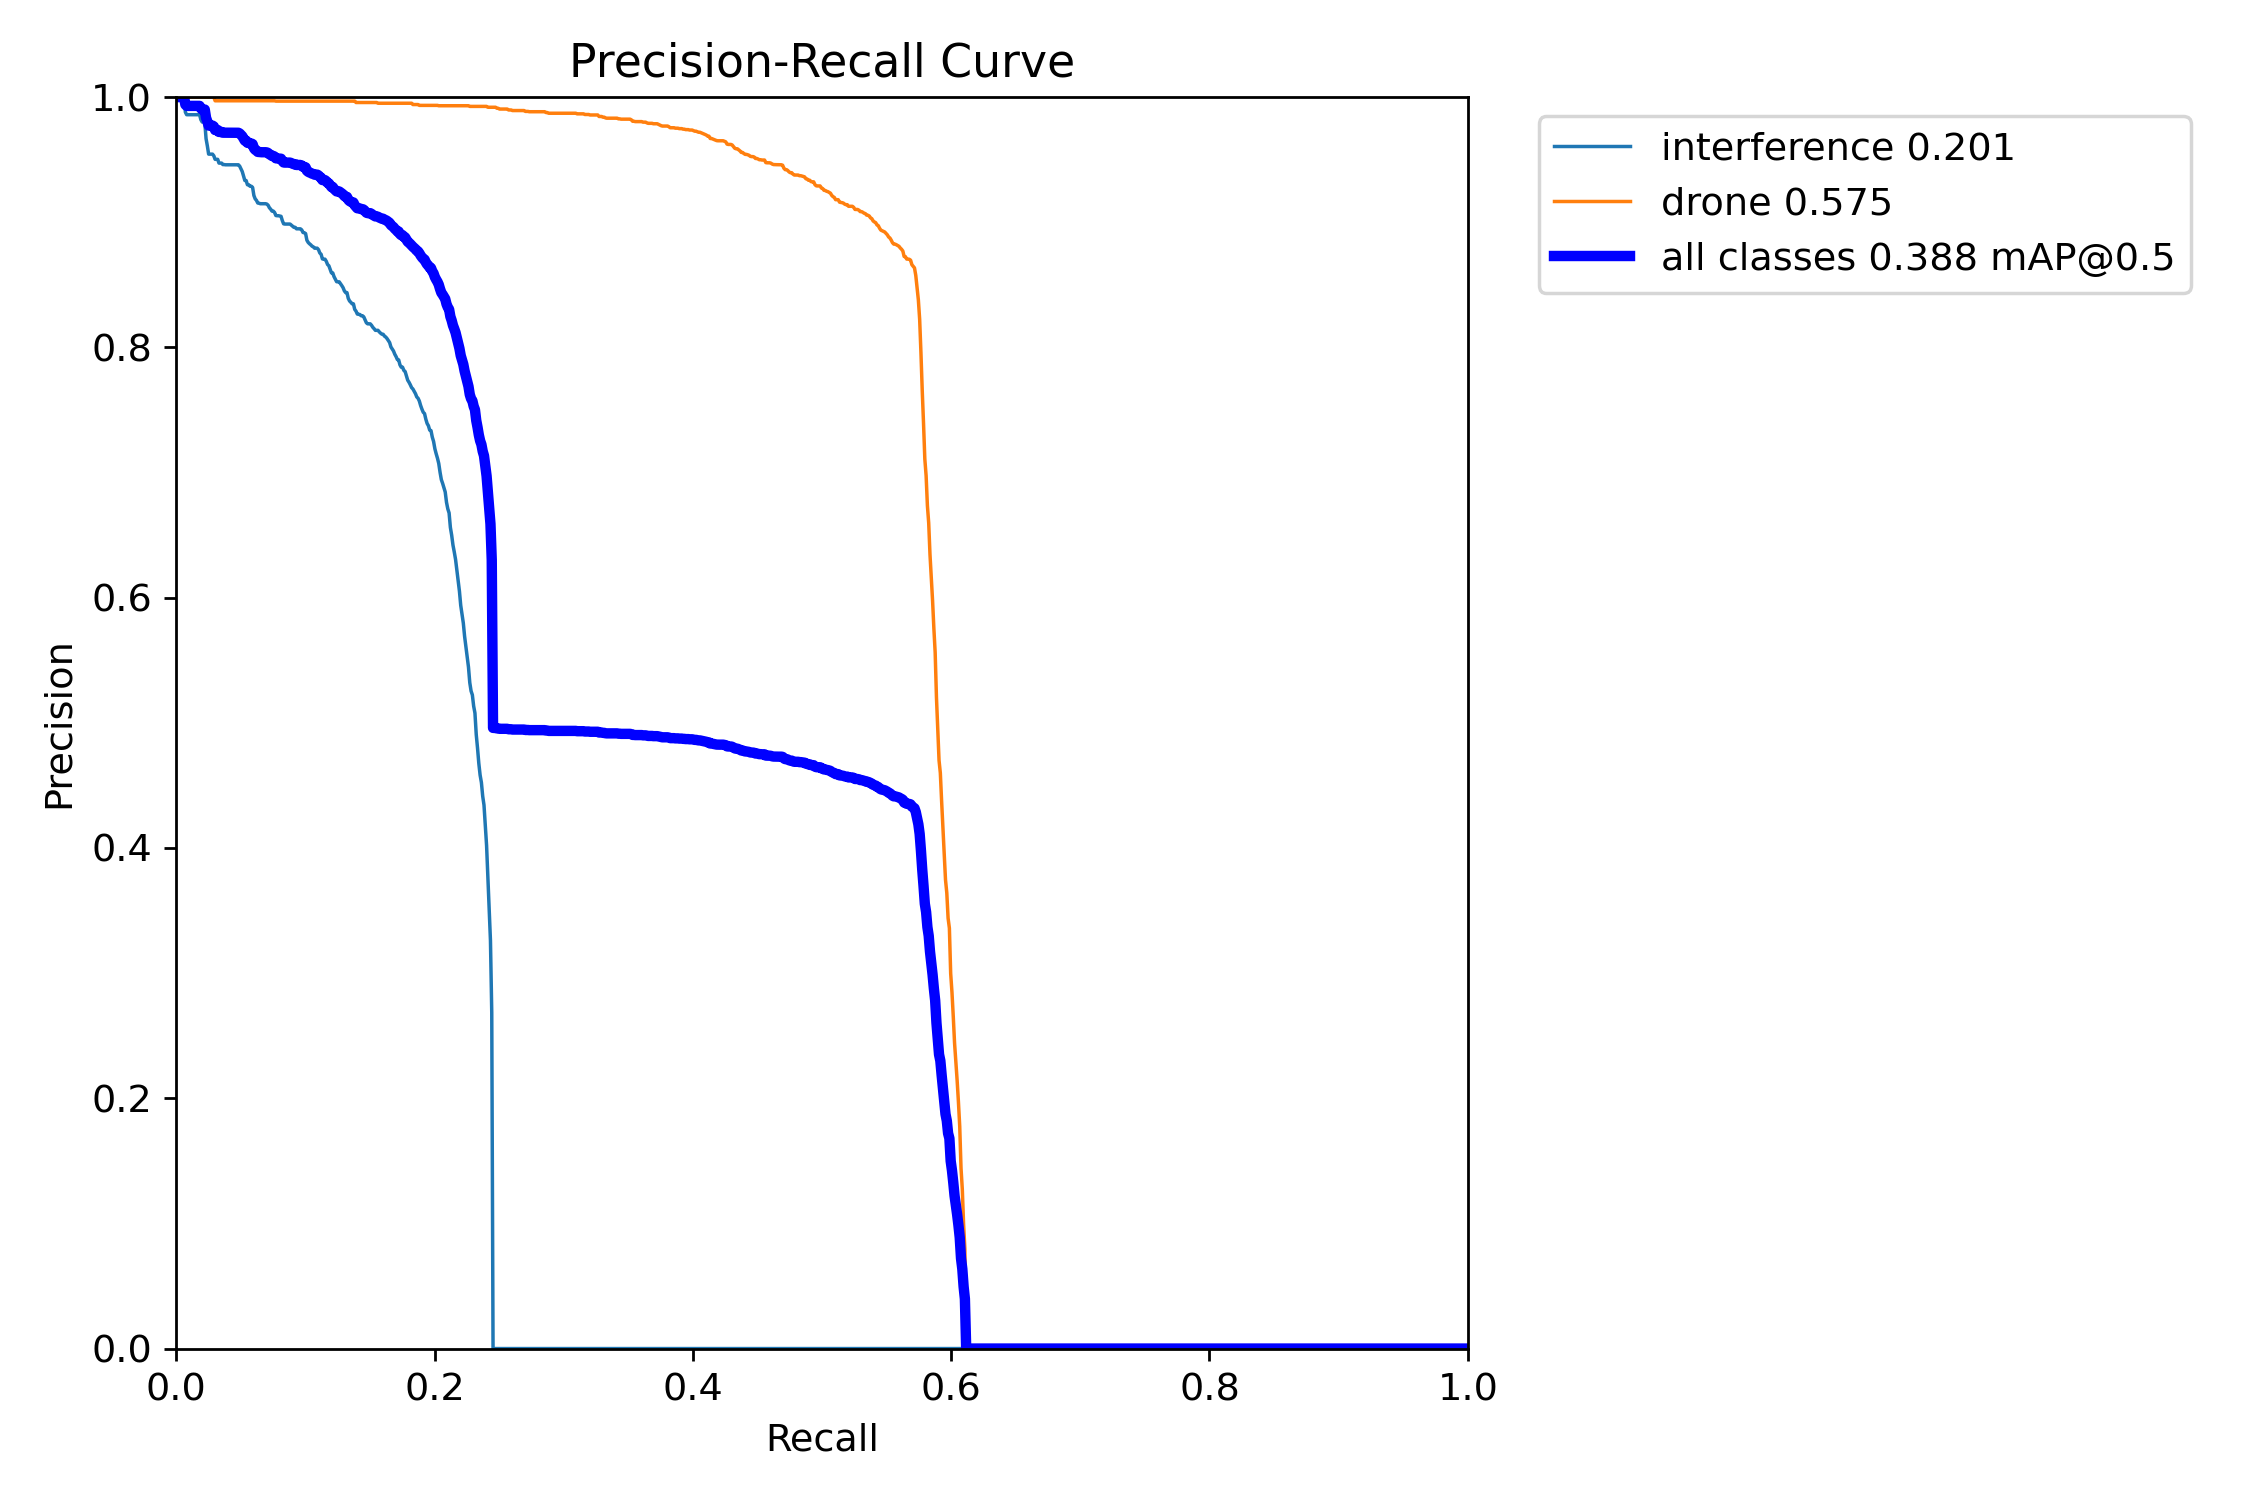
\includegraphics[width=0.85\textwidth]{figuras/resultados/BoxPR_curve.png}
    \caption{Curva precisión-recall del detector YOLOv8n sobre el conjunto de prueba. Cada punto corresponde a un umbral de confianza distinto. La clase \emph{drone} mantiene una precisión elevada en un rango de recall más amplio que \emph{interference}, lo que refleja la mayor homogeneidad de las ráfagas OcuSync respecto a las interferencias heterogéneas.}
    \label{fig:box_pr_curve}
\end{figure}

La \cref{fig:box_f1_curve} complementa la anterior mostrando el F1 en función del umbral de confianza. Esta curva permite identificar directamente el umbral que maximiza el F1 para cada clase o para el sistema global, y es la herramienta principal para seleccionar el punto de operación del sistema de detección. El máximo global se alcanza con umbrales de confianza bajos (en torno a 0,10-0,20), lo que indica que el detector asigna puntuaciones moderadas a una fracción relevante de ráfagas reales. En el experimento P3 se explotan explícitamente distintos valores de este umbral para determinar el punto de operación del clasificador de presencia.

\begin{figure}[htbp]
    \centering
    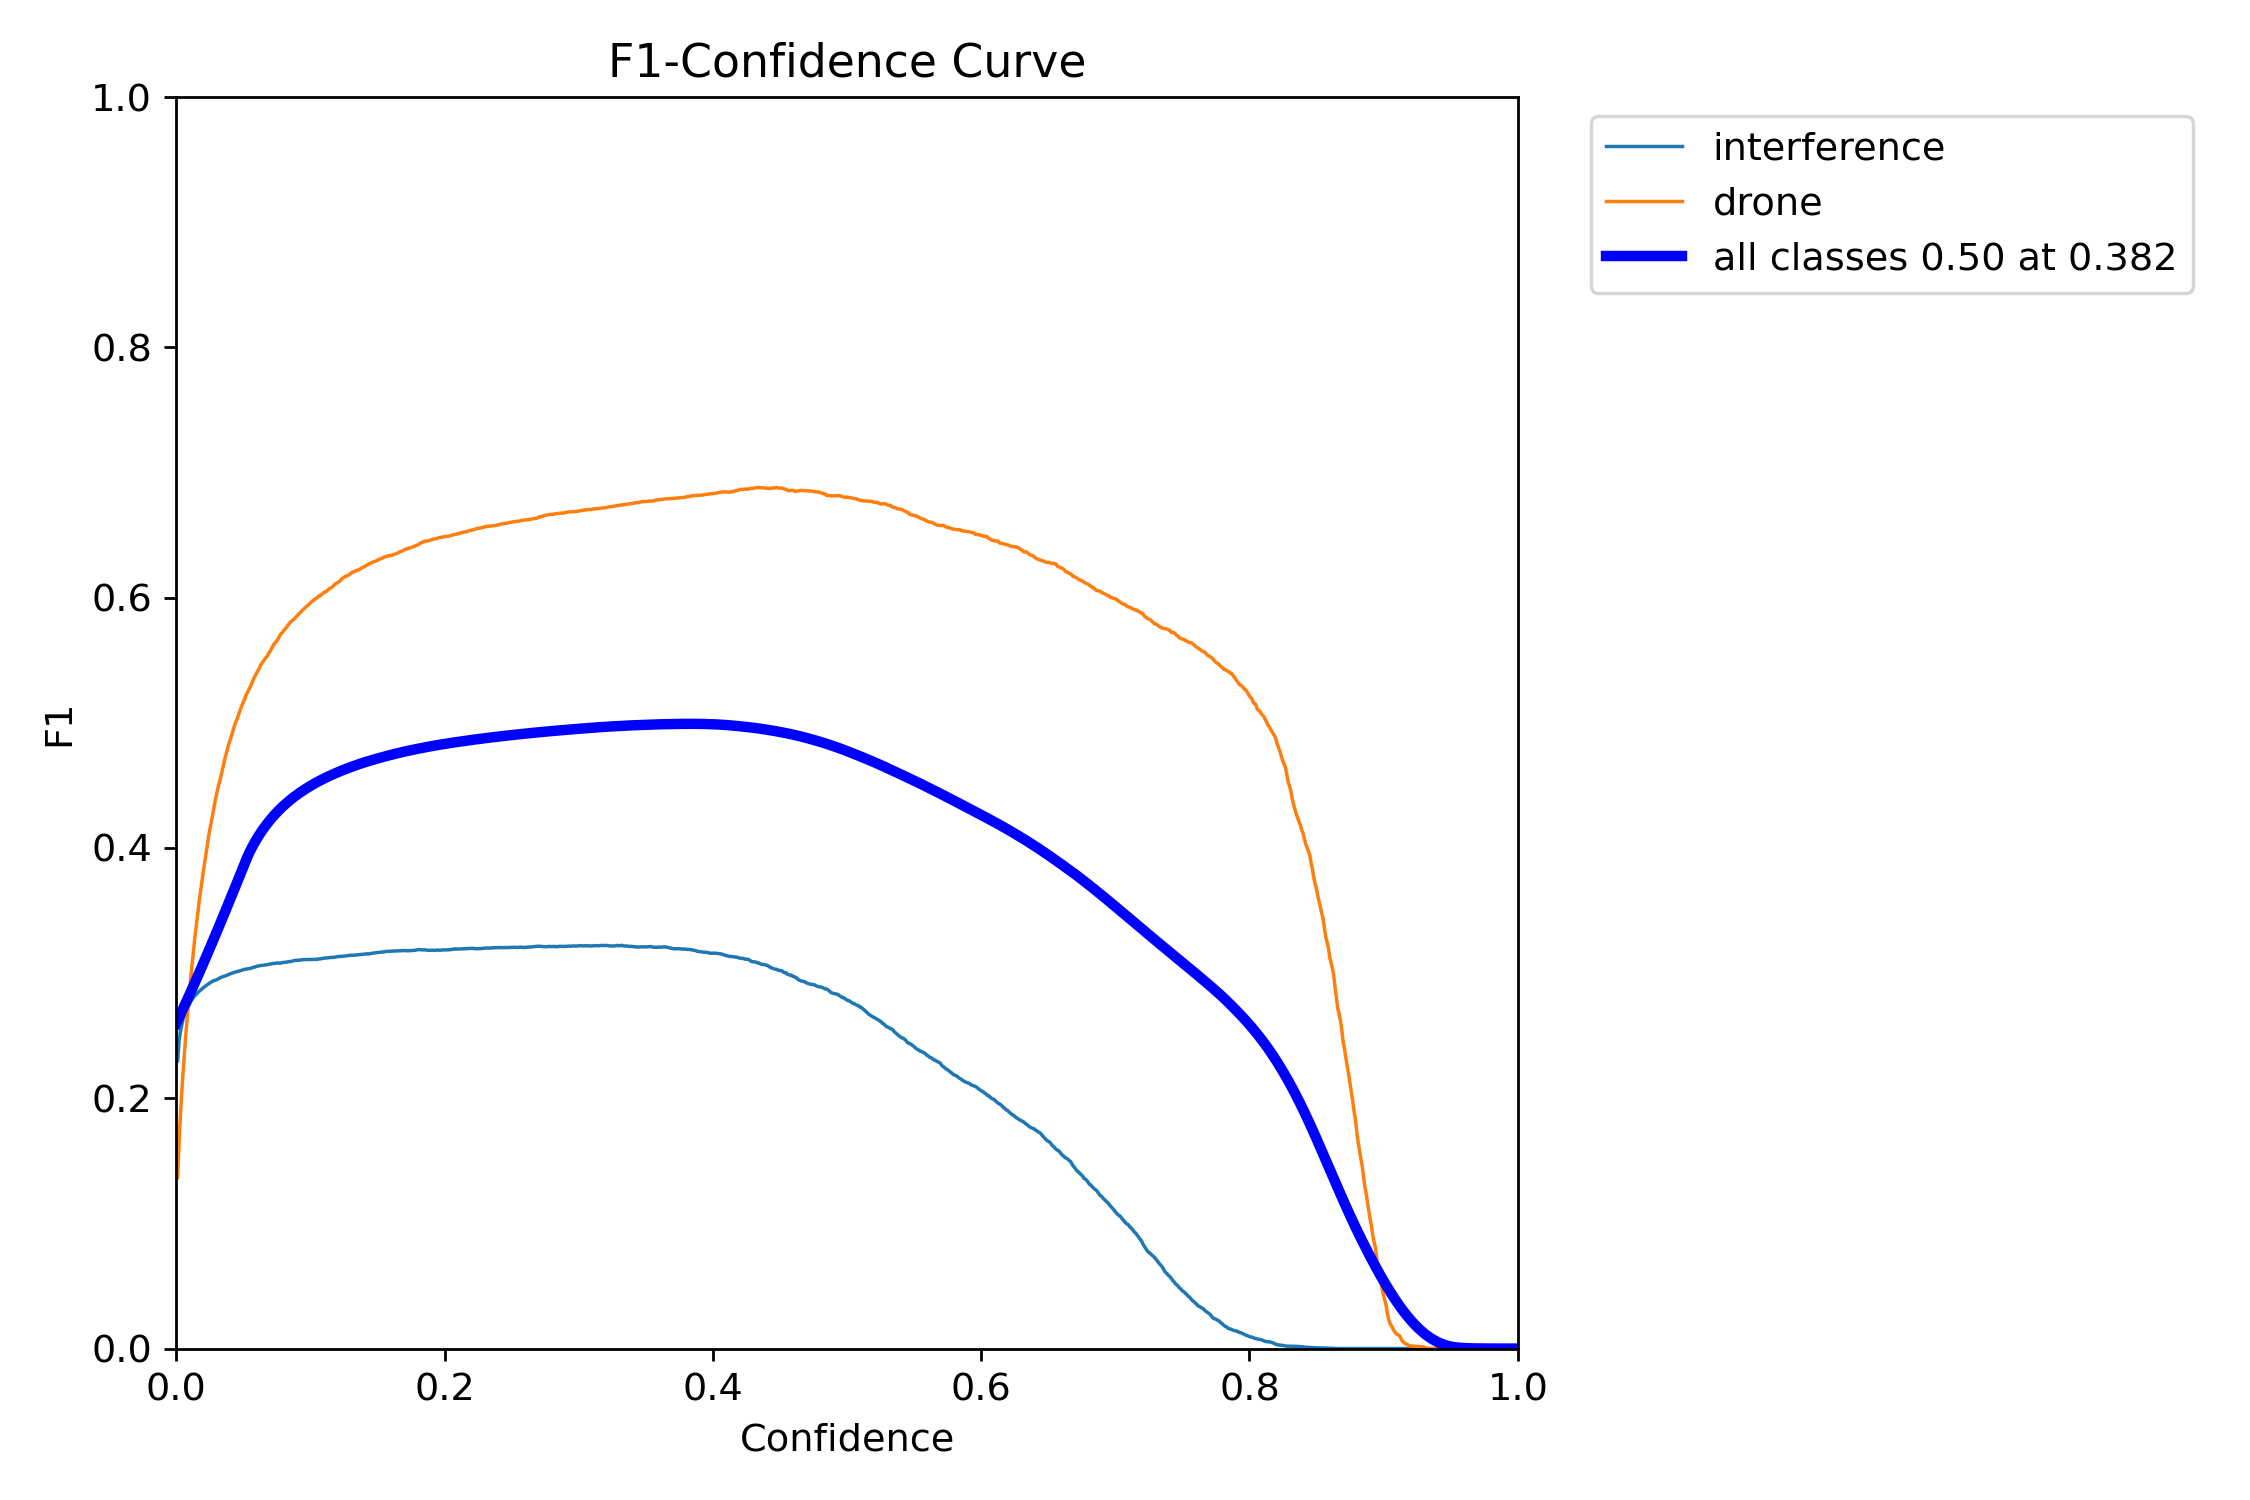
\includegraphics[width=0.85\textwidth]{figuras/resultados/BoxF1_curve.png}
    \caption{Curva F1-confianza del detector YOLOv8n. El eje horizontal representa el umbral de confianza mínimo para retener una detección, y el eje vertical el F1 resultante. El máximo global se alcanza con un umbral bajo, lo que indica que bajar el umbral recupera ráfagas reales sin penalizar excesivamente la precisión.}
    \label{fig:box_f1_curve}
\end{figure}

\FloatBarrier
\paragraph{Ejemplos cualitativos.}

Las \cref{fig:val_labels,fig:val_pred} comparan las etiquetas de referencia con las predicciones del modelo sobre un mismo lote de validación, permitiendo verificar visualmente la coherencia entre las métricas agregadas y el comportamiento sobre espectrogramas concretos.

\begin{figure}[htbp]
    \centering
    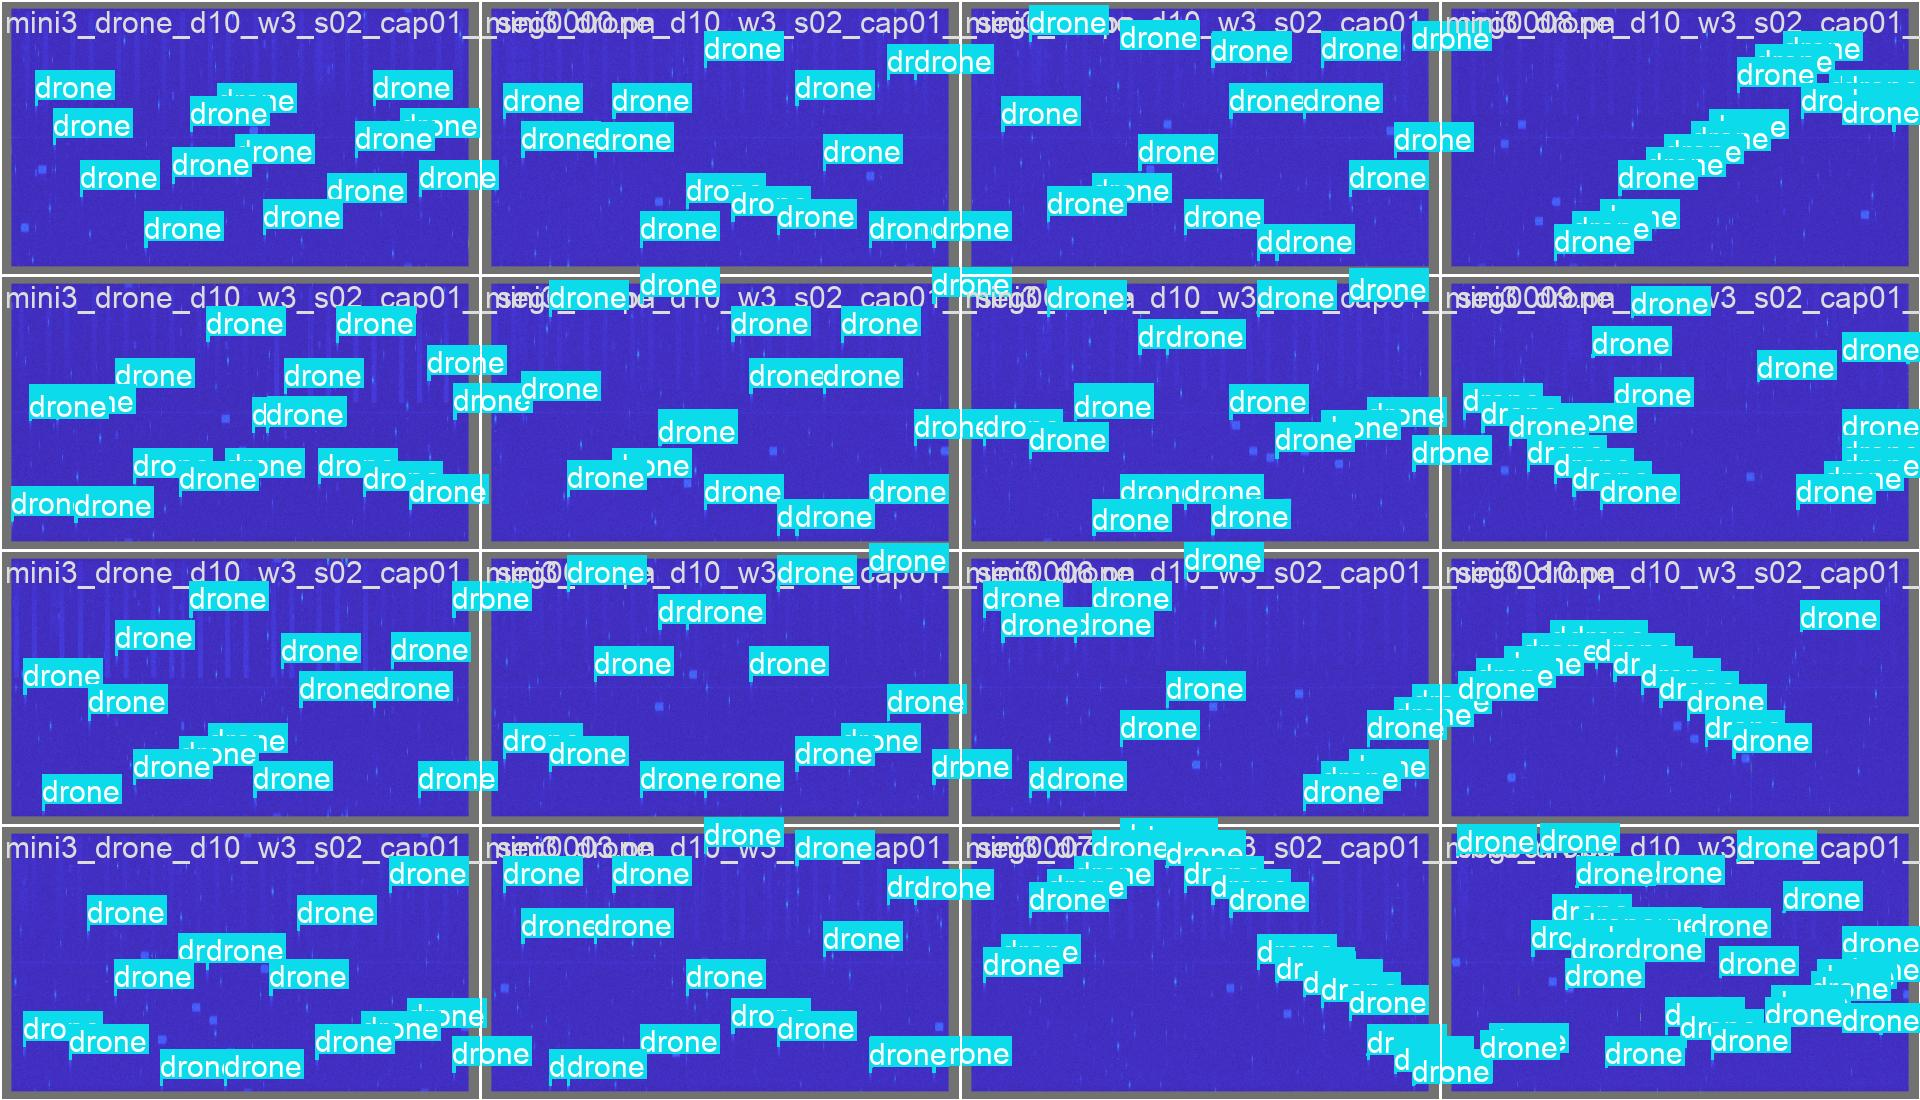
\includegraphics[width=0.9\textwidth]{figuras/resultados/val_batch0_labels.jpg}
    \caption{Etiquetas de referencia (\emph{ground truth}) sobre un lote de validación de capturas de dron. Cada caja delimita una ráfaga FHSS de OcuSync generada por el auto-etiquetado.}
    \label{fig:val_labels}
\end{figure}

\begin{figure}[htbp]
    \centering
    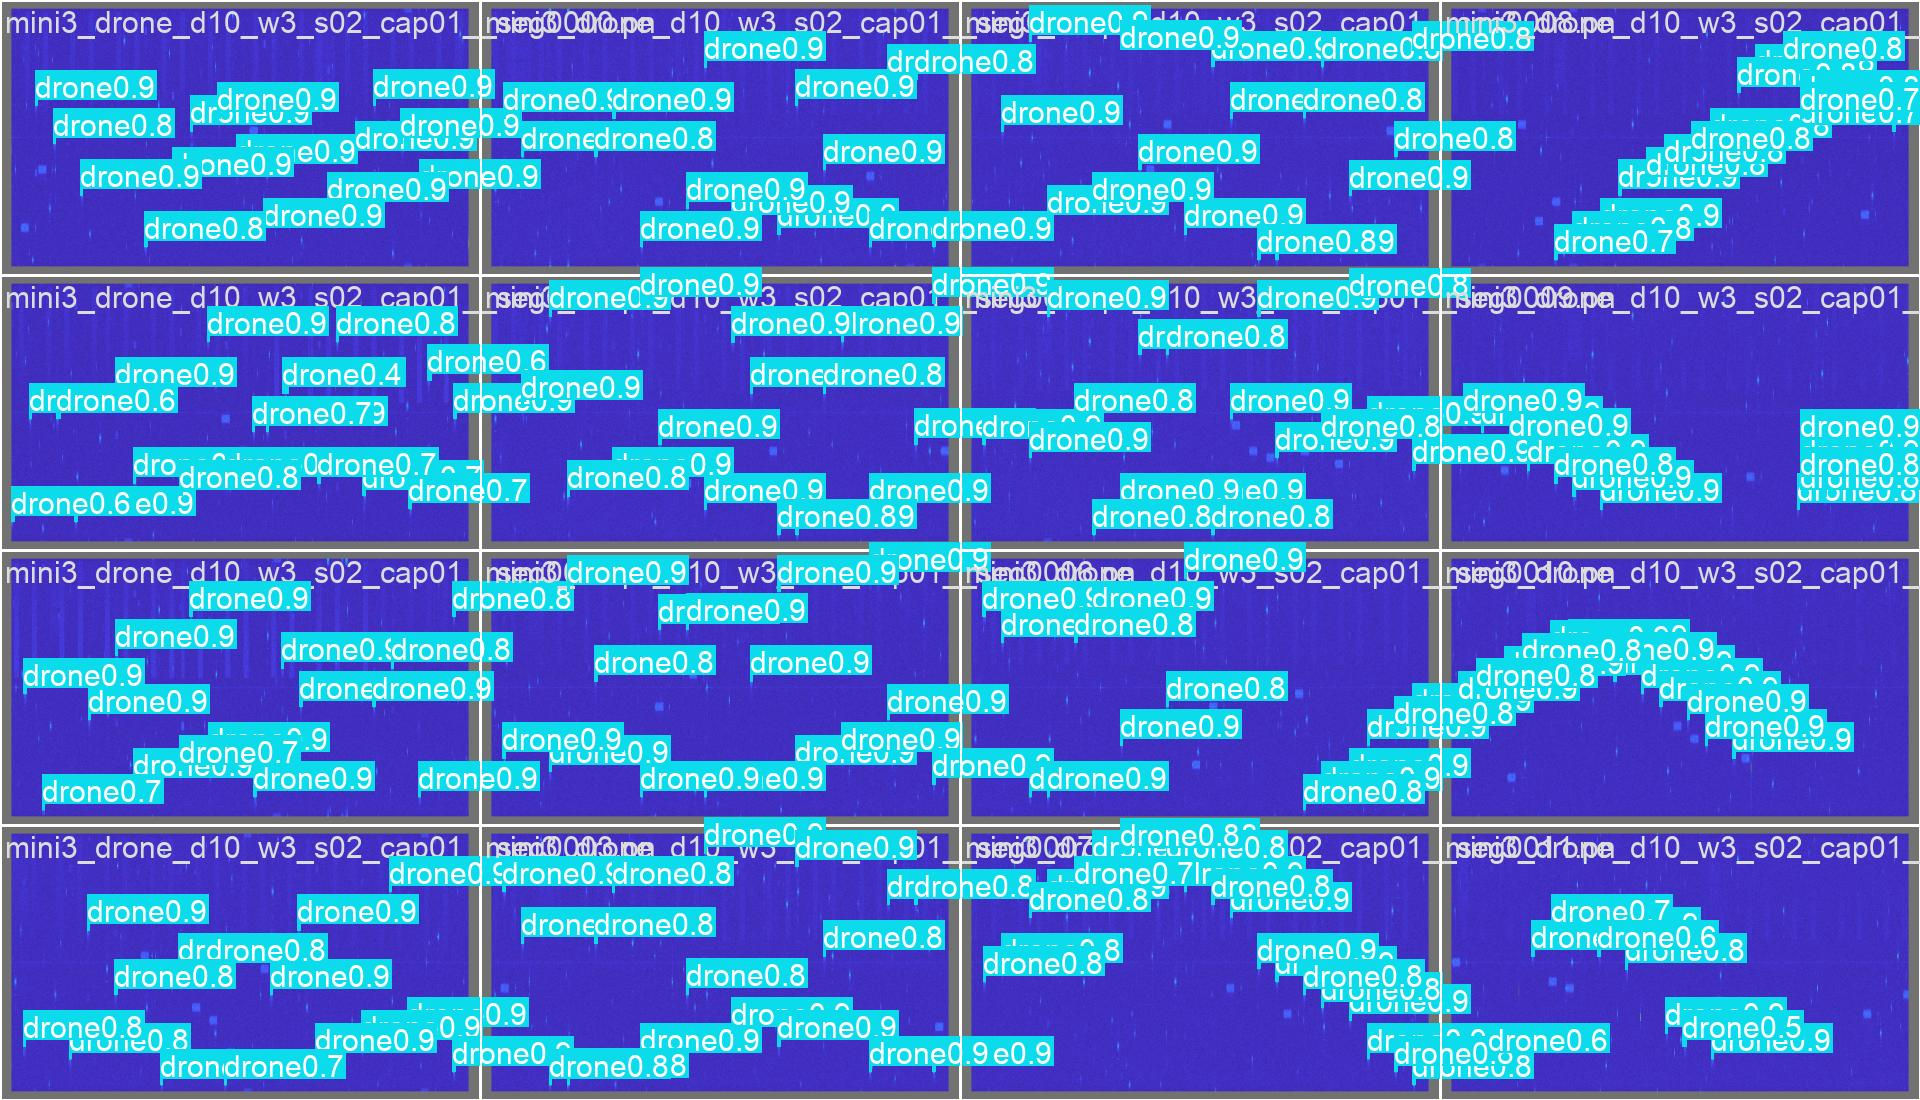
\includegraphics[width=0.9\textwidth]{figuras/resultados/val_batch0_pred.jpg}
    \caption{Predicciones del detector YOLOv8n sobre el mismo lote, con su puntuación de confianza asociada. Las cajas predichas se superponen sobre las mismas ráfagas FHSS que indican las etiquetas de referencia de la \cref{fig:val_labels}, con confianzas típicas entre 0,6 y 0,9. No aparecen cajas sobre regiones de fondo vacío: no hay falsos positivos.}
    \label{fig:val_pred}
\end{figure}

La comparación entre ambas figuras muestra que las cajas predichas se sitúan sobre las mismas ráfagas que las etiquetas de referencia. La densidad de cajas predichas es inferior a la de referencia, lo que es coherente con el recall de 0,39: el modelo no recupera todas las ráfagas etiquetadas. No aparecen, en cambio, cajas sobre regiones del espectrograma sin señal: no hay falsos positivos.

\FloatBarrier
\subsection{Interpretabilidad mediante EigenCAM}
\label{sec:eigencam}

Las métricas anteriores cuantifican el rendimiento del detector pero no revelan en qué características del espectrograma se apoya para inferir sus decisiones. Esta información es relevante para la auditabilidad del sistema: en aplicaciones de vigilancia, un detector debe poder justificar sus predicciones de forma verificable. Con este objetivo se aplica EigenCAM para analizar qué regiones del espectrograma activan internamente la red.

EigenCAM extrae las activaciones de la capa del cuello de YOLOv8 responsable de detectar objetos de tamaño pequeño y calcula su primera componente principal, produciendo un mapa de calor sobre el espectrograma. Al operar directamente sobre activaciones --- y no sobre gradientes respecto a ninguna clase objetivo ---, el mapa refleja las regiones que generan respuestas fuertes y coherentes en la red con independencia de la clase predicha.

\begin{figure}[htbp]
    \centering
    \begin{subfigure}[b]{0.48\textwidth}
        \centering
        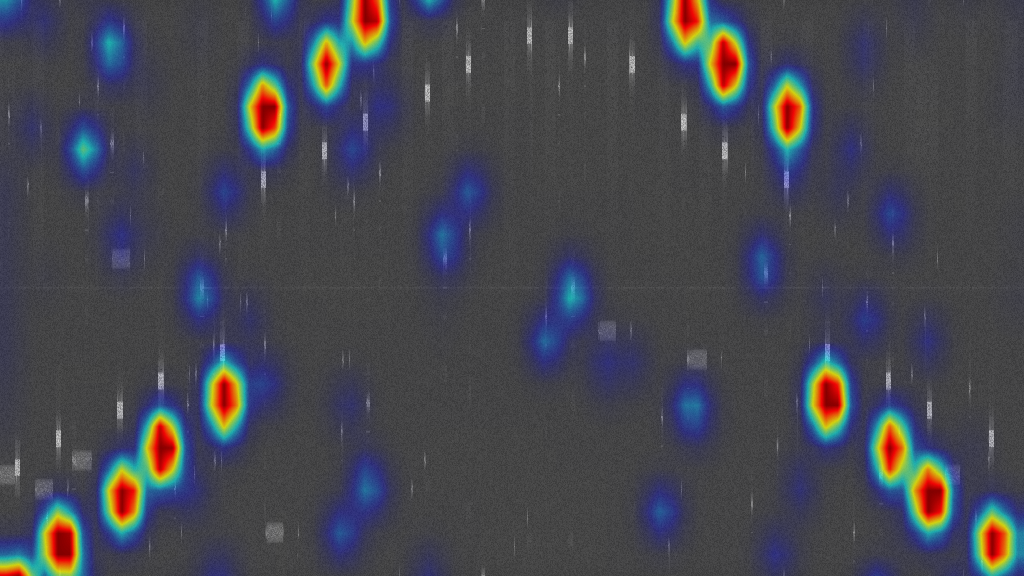
\includegraphics[width=\textwidth]{figuras/resultados/cam_drone_00.png}
        \caption{Captura con dron (protocolo OcuSync).}
        \label{fig:eigencam_drone}
    \end{subfigure}
    \hfill
    \begin{subfigure}[b]{0.48\textwidth}
        \centering
        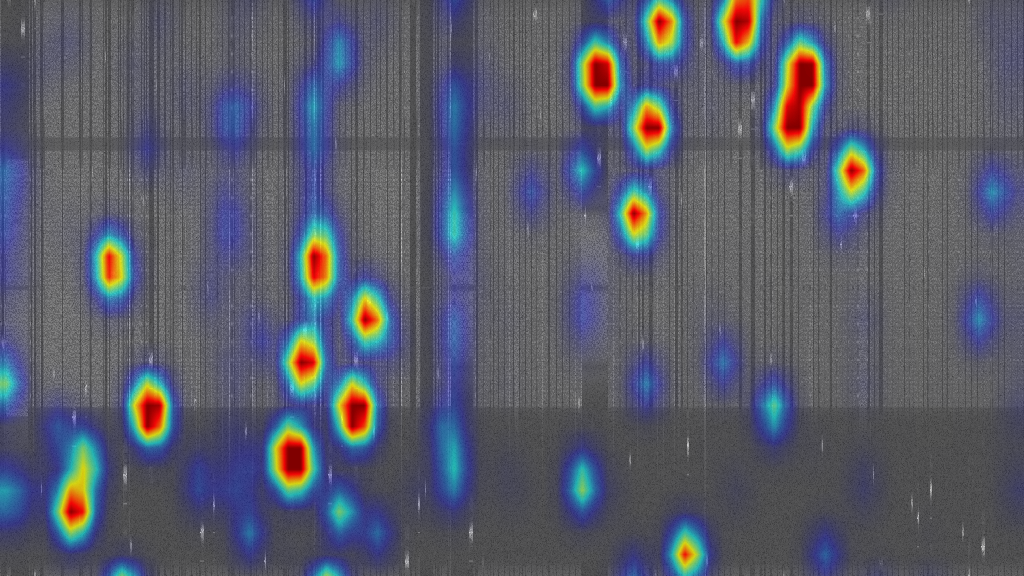
\includegraphics[width=\textwidth]{figuras/resultados/eigencam_interference.png}
        \caption{Captura de interferencia (WiFi/Bluetooth).}
        \label{fig:eigencam_interference}
    \end{subfigure}
    \caption{Mapas de saliencia EigenCAM del detector YOLOv8n sobre dos espectrogramas de prueba. El espectrograma subyacente se muestra en escala de grises y el color indica la intensidad de activación (rojo = alta, azul = baja). En la captura de dron, los focos de activación coinciden con las posiciones de las ráfagas OcuSync que las etiquetas de referencia de la \cref{fig:val_labels} delimitan como \emph{drone}. En la captura de interferencia, la activación recae sobre las estructuras WiFi y Bluetooth activas.}
    \label{fig:eigencam}
\end{figure}

La \cref{fig:eigencam} muestra los resultados para dos espectrogramas representativos del conjunto de prueba. En la captura de dron (\cref{fig:eigencam_drone}), los focos de calor son estructuras compactas que coinciden espacialmente con las ráfagas FHSS de OcuSync: las mismas posiciones que las etiquetas de referencia de la \cref{fig:val_labels} identifican como \emph{drone}. En la captura de interferencia (\cref{fig:eigencam_interference}), la activación recae sobre las columnas WiFi y las ráfagas Bluetooth. En ningún caso se producen activaciones sobre regiones de fondo vacío, lo que confirma que las respuestas de la red se asocian a estructuras de señal y no a artefactos del contexto de captura.

\FloatBarrier
Cabe señalar que EigenCAM no discrimina entre clases: el mapa indica únicamente dónde existen activaciones fuertes, no si estas corresponden a \emph{drone} o a \emph{interference}. La capacidad de separar ambas clases se sustenta en la ausencia de confusión cruzada de la \cref{fig:confusion_matrix_normalized}, y se refuerza cuantitativamente con el experimento de robustez de la \cref{sec:bloque_clasificacion}.
